\documentclass[../main.tex]{subfiles}
\begin{document}
\onlyinsubfile{
\setcounter{chapter}{0}
}
\notinsubfile{}
\section{Een andere qubit}\label{sec:anderqubit}

\marginpar{\hfill\fbox{
\begin{minipage}[t]
{0.9\marginparwidth}naam:\hfill\vspace{1cm}
\end{minipage}
}}
\marginpar{\hfill\fbox{
\begin{minipage}[t]
{0.9\marginparwidth}klas:\hfill\vspace{1cm}
\end{minipage}
}}
\marginpar{\hfill\fbox{
\begin{minipage}[t]
{0.9\marginparwidth}datum:\hfill\vspace{1cm}
\end{minipage}
}}
\begin{center}
\leavevmode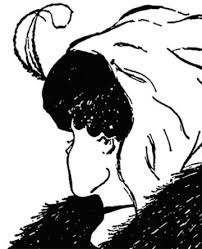
\includegraphics[width=0.5\textwidth]{./img/ovjv.png}
 \captionof{figure}{Oude vrouw jonge vrouw.
\label {fig:wbovjv}}
\end{center}

\nogdoen{onderdeel van opdracht hardware?}Er zijn veel soorten qubits. Naast het foton is de elektronspin de meest bekende.  Begin twintigste eeuw werd veel bekend over het gedrag van elektronen in een magnetisch veld. Elektronen zouden zich gedragen als een kompasnaald.  Later werd duidelijk dat dat beeld veel te eenvoudig is.  Gelukkig is niet veel kennis over het fysische gedrag van qubits nodig om een quantumcomputer te kunnen programmeren.  Je kunt over de software praten zonder de hardware te kennen. Maar het is wel nodig om iets te weten over de  eigenschappen die alle  qubits gemeen hebben. Om goed zicht te krijgen op die eigenschappen zullen we gebruikmaken van een denkbeeldig qubit.  En dan is dat beeld van een kompasnaald zo gek nog niet.

\paragraph{Een denkbeeldige qubit}
Een denkbeeldig apparaat biedt ruimte aan een kompasnaald in een magnetisch veld. De richting van het  magnetisch veld  kan worden ingesteld met een instelknop.  Om de kompasnaald waar te nemen is een knop aanwezig die moet worden ingedrukt. De kompasnaald heeft de quantumeigenschap dat hij maar in twee toestanden kan worden waargenomen. Bekijk figuur~\ref{fig:apparaat}.


\begin{center}
\leavevmode
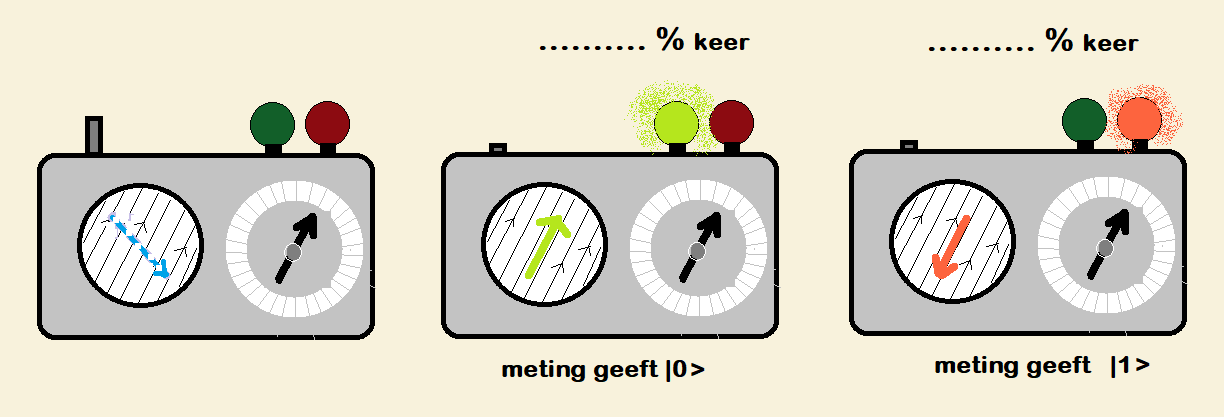
\includegraphics[width=\textwidth]{./img/apparaat.png}
\captionof{figure}{Een denkbeeldig apparaat. Een kompasnaald in een magnetisch veld kan bij uitlezing twee toestanden hebben: met het veld mee (groene lamp aan) of tegen het veld in (rode lamp aan).  Hier zal de rode lamp het vaakst branden.
\label{fig:apparaat}}
\end{center}


Het meetapparaat kan twee toestanden van een qubit onderscheiden. Als het qubit zich in toestand $\ket{0}$ bevindt zal bij uitlezing altijd de groene lamp branden. Bevindt het qubit zich in toestand $\ket{1}$ dan zal altijd de rode lamp branden. Bevindt het qubit zich in een andere toestand dan zal soms de rode lamp branden, soms de groene lamp branden.

De hier afgebeelde qubit lijkt het meeste op wat genoemd wordt de \textit{elektronspin}. Een elektron in een magneetveld gedraagt zich als een kompasnaald die maar twee standen kent. De ene is de toestand waarbij de kompasnaaldrichting dezelfde richting heeft als het magneetveld. Dat wordt hier de toestand $\ket{0}$ genoemd. Maar er is ook een toestand waarbij de kompasnaaldrichting tegengesteld is aan het magneetveld. Dat is dan de toestand $\ket{1}$. Elektronen hebben in toestand$\ket{1}$ iets meer energie dan in toestand $\ket{0}$. Je zult arbeid moet verrichten om het elektron van toestand $\ket{0}$ naar toestand$\ket{1}$te brengen. 

Bij de elektronspin is het even oppassen geblazen dat je de spinrichting niet verwart met de toestandsvector. Om dat duidelijk te maken is in figuur~\ref{fig:kwadrant} de eenheidscirkel afgebeeld maar nu met de drie toestandsvectoren die horen bij de situatie in figuur~\ref{fig:apparaat}. De hoek tussen de rode en groene spinrichting is \SI{180}{\degree}. De hoek tussen de toestandsvectoren van de twee basistoestanden is \SI{90}{\degree}.  De hoeken die bij spinrichtingen (de richting van de kompasnaald) horen zijn 2x zo groot als de hoeken tussen de toestandsvectoren. De hoek tussen de blauwe en de rode spinrichting is ongeveer \SI{60}{\degree}. Die tussen de beide toestandsvectoren is dan \SI{30}{\degree}. De componenten van de blauwe toestandsvector zijn dan $\tfrac{1}{2}$ en $\tfrac{1}{2}\sqrt{3}$. Daarmee kunnen dan de toestandsvectoren worden ingetekend in de eenheidscirkel. Daarmee kunnen we dan de toestandsvectoren intekenen in de eenheidscirkel.

\begin{flushleft}
%\leavevmode
\begin{minipage}{.45\textwidth}
\def\ojfrangle{0}
\def\ojobangle{60}
\def\ojscale{.75}
\begin{tikzpicture}%
\begin{scope}[scale=\ojscale, rotate=\ojfrangle]
  \draw[thin,gray!40] (-0.1,-0.1) grid (5,5);
  \draw[-stealth] (-0.1,0)--(5*cos{\ojobangle},0) 
        node[midway, below, xshift=0]
        {${\scriptstyle{\alpha}}$};
%        {${\scriptstyle\braket{0}{\Psi}}$};
  \draw[-stealth] (0,-0.1)-- (0,5*sin{\ojobangle}) 
        node[midway, left, yshift=0]
        {${\scriptstyle{\beta}}$};
%        {${\scriptstyle\braket{1}{\Psi}}$};
  \node[above] at (0,5) {$\ket{1}$};
  \node[right] at (5,0) {$\ket{0}$};
  \draw[line width=.1pt ,black] ([shift=(0:5)]0,0) arc (0:90:5);
  \draw[thick, red, -stealth](0,0)--(90:5);
  \draw[thick, green, -stealth](0,0)--(0:5);
  \draw[thick, blue, -stealth](0,0)--(\ojobangle:5)
       node[label={[above, right]$\ket{\Psi}$}] (p){};
  \draw[line width=1pt,dotted] (0,5*sin{\ojobangle}) -- (p);
  \draw[line width=1pt,dotted] (p)--(5*cos{\ojobangle},0);
\end{scope}
\end{tikzpicture}
\end{minipage}%
\hfill
\begin{minipage}{.5\textwidth}
 \captionof{figure}{Drie Toestandsvectoren. Toestand $\ket{\Psi}$ heeft meer overlap met $\ket{1}$ dan met $\ket{0}$.\label{fig:kwadrant}}
\end{minipage}
\end{flushleft}


De co\"effici\"ent $\alpha$ is ongeveer gelijk aan \num{0.5}. De kans dat de groene lamp gaat branden is dan \num{0.25} ofwel \SI{25}{\percent}. De kans dat de rode lamp gaat branden moet dan \SI{75}{\percent} zijn. De co\"effici\"ent $\beta$ is dan $\sqrt{0.75}=0.87$. De co\"effici\"enten $\alpha$ en $\beta$ worden amplitudes genoemd. 

\paragraph{Uitlezing}
\marginpar{\footnotesize{Bij de proef van Young geeft \'e\'en foton op het scherm niet genoeg informatie om een een enkel- of dubbelspleet te herkennen, en  \'e\'en blik op het plaatje wil niet zeggen dat er alleen een oude vrouw is afgebeeld.}}
Een waarneming in de quantumwereld verlooptt wezenlijk anders dan in de klassiek wereld. De stand van een thermometer kun je zo aflezen zonder dat de temperatuur van de kamer verandert, maar in de quantumwereld kun je niet meten zonder het object te verstoren. De toestand is na een meting verloren. Om een indruk te krijgen van een quantumsysteem is een meting niet voldoende. Denk aan de spleetexperiemnten van Young en aan het experiment met de oude en de jonge vrouw.
Er moet altijd statistiek worden bedreven. Hoe heet deze module ook al weer? 
Als een qubit eenmaal is uitgelezen dan is de toestand van het qubit ook verloren. De toestand $\ket{\Psi}$ is overgegaan in een basistoestand $\ket{0}$ of $\ket{1}$. Meten is projecteren als je naar figuur~\ref{fig:kwadrant} kijkt.  
Deze twee wetmatigheden (de meting vernietigt de quantumtoestand, en de meting gaat volgens een kansproces) betekenen dat het qubit een aantal maal opnieuw geprepareerd zal moeten worden in de toestand $\ket{\Psi}$.
Het uitlezen is dus onomkeerbaar, \textit{irreversibel}. Het proces kan niet ongedaan worden gemaakt. Dat betekent dat klonen of kopi\"eren van een file bij de quantumcomputer niet mogelijk is. Dat lijkt een probleem, maar het is juist  een unieke eigenschap van quantumcomputers die encryptie absoluut veilig maakt (zie werkblad~\ref{sec:wbBB84}). 

\begin{opdracht}\label{opd:apparaat}
Iemand draait aan de instelling van het meetapparaat in figuur~\ref{fig:kwadrant} en herhaalt het experiment. De toestand van het qubit is niet gewijzigd. Nu blijkt in \SI{60}{\percent} van de gevallen de groene lamp te branden en in \SI{40}{\percent} de rode lamp.

\begin{enumerate}
\item Bereken de co\"effici\"enten $\alpha$ en $\beta$.
\item Hoeveel graden is de wijzer gedraaid en in welke richting?
\end{enumerate}
\end{opdracht}
\begin{antwoord}[-4cm]
Hoek van de toestandvector was: $tan^{-1}\tfrac{\beta}{\alpha}= tan^{-1}\tfrac{\tfrac{1}{2}\sqrt{3}}{0.5}\implies \SI{60}{\degree}$
Voor de wijzer geldt de dubele hoek: (dit is wel verwarrend)

nieuwe situatie: 
$\alpha^2=\num{0.6} \implies \alpha=\tfrac{\sqrt{3}}{\sqrt{5}}$\\
$\beta^2=\num{0.4} \implies \beta=\tfrac{\sqrt{2}}{\sqrt{5}}$\\

Er zijn vier mogelijkheden voor de nieuwe toestand, in het eerste kwadrant:
$tan^{-1}\sqrt{\tfrac{\beta}{\alpha}} \implies \SI{50.8}{\degree}$
De stand van de naald gaat met de dubbele hoek: $\SI{102}{\degree}$ dus verdraaid over \nogdoen{\SI{-9.2}{\degree}}
\end{antwoord}

\nogdoen{Oeps ik heb geen rekening gehouden met de toestandsvector (factor twee) Guido?}




\paragraph{Keuze van de basis}

Het meetapparaat van figuur~\ref{fig:apparaat} bevat een wijzer waarmee de instelling van het apparaat kan worden gewijzigd. In dit geval wordt het magnetisch veld van het meetapparaat gekanteld. Is zo'n wijzer zinvol? Als de uit te lezen qubits van buitenaf komen, geprepareerd met een andere basis dan kan dat heel zinvol zijn. Stel maar eens dat de qubits door apparaat A zijn geprepareerd in de toestand $\ket{0}$ dan zou bij een willekeurige instelling van het uitleesapparaat vermoedelijk een superpositie worden uitgelezen. Zo'n wijzer op het uitleesapparaat zou dan heel nuttig zijn. Je draait net zo lang aan de wijzer tot de groene lamp permanent brandt.
Maar er zijn meer voordelen. Er zijn toepassingen waarbij meer dan \'e\'en basis nodig is. Een van die toepassingen wordt besproken in hoofdstuk 4.
Daarbij wordt gebruik gemaakt van de standaardbasis maar ook van de diagonale basis. In figuur~\ref{fig:BB84base} zijn de beide bases weergegeven.  

\iffalse
\begin{flushleft}
%\leavevmode
\begin{minipage}{.35\textwidth}
\def\ojfrangle{0}
\def\ojobangle{45}
\def\ojscale{.45}
\begin{tikzpicture}%
\begin{scope}[scale=\ojscale, rotate=\ojfrangle]
  \draw[thin,red!40] (-5,-5) grid (5,5);
  \draw[line width=.1pt ,black!30] ([shift=(-90:5)]0,0) arc (-90:180:5);
  \draw[-stealth,, red!40] (-0.1,0)--(5,0) node[below, red, xshift=10]{${\scriptstyle\ket{H}}$};
  \draw[-stealth, red!40] (0,-0.1)-- (0,5) node[left, red, yshift=0]{${\scriptstyle\ket{V}}$};
%  \draw[line width=.1pt ,black] ([shift=(0:5)]0,0) arc (0:90:5);
  \draw[thick, red, -stealth](0,0)--($cos(\ojobangle-\ojfrangle)*(5,0)$) node(x){};
  \draw[thick, red, -stealth](0,0)--($sin(\ojobangle-\ojfrangle)*(0,5)$) node(y){};
  \draw[thick, black!50, -stealth](0,0)--(\ojobangle-\ojfrangle:5) node (p){};
  \draw[loosely dashed] (x)--(p);
  \draw[loosely dashed] (y)--(p);
\end{scope}
\def\ojfrangle{-45}
\begin{scope}[scale=\ojscale,  rotate=\ojfrangle]
  \draw[thin,green!40!lightgray] (-5,-5) grid (5,5);
  \draw[-stealth, green!40!gray] (-0.1,0)--(5,0) node[right,  xshift=-3, yshift=-3]{${\scriptstyle\ket{-}}$};
  \draw[-stealth,green!40!gray] (0,-0.1)-- (0,5) node[above left,  xshift=13]{${\scriptstyle\ket{+}}$};
%  \draw[line width=.1pt ,black] ([shift=(0:5)]0,0) arc (0:90:5);
  \draw[thick, black, -stealth](0,0)--($cos(\ojobangle-\ojfrangle)*(5,0)$) node(x){};
  \draw[thick, black, -stealth](0,0)--($sin(\ojobangle-\ojfrangle)*(0,5)$) node(y){};
  \draw[thick, black!50, -stealth](0,0)--(\ojobangle-\ojfrangle:5) node (p){};
  \draw[ dotted] (x)--(p);
  \draw[ dotted] (y)--(p);
\end{scope}
\end{tikzpicture}
\end{minipage}%
\hfill
\begin{minipage}{.45\textwidth}
%\[\begin{aligned}
%\ket{+}&=\tfrac{1}{2}\sqrt{2}\ket{H}+\tfrac{1}{2}\sqrt{2}\ket{V}\\
%\ket{-}&=\tfrac{1}{2}\sqrt{2}\ket{H}-\tfrac{1}{2}\sqrt{2}\ket{V}\\ 
%\ket{H}&=\tfrac{1}{2}\sqrt{2}\ket{+}+\tfrac{1}{2}\sqrt{2}\ket{-}\\
%\ket{V}&=\tfrac{1}{2}\sqrt{2}\ket{+}-\tfrac{1}{2}\sqrt{2}\ket{-}\\
%\end{aligned}\]%subtiel veel minder whitespace
\captionof{figure}{In de standaardbasis (rood) wordt de blauwe toestandsvector genoteerd als $\ket{\Psi} =\alpha\ket{0}+\beta\ket{1}$ waargenomen. In de diagonale basis  (groen) als $\ket{\Psi} =\gamma\ket{0}+\delta\ket{1}$ waargenomen.}\label{fig:BB84base}
\end{minipage}
%\caption{E\'en vector in standaardbasis (rood) en diagonale basis.}\label{fig:hvad}
%\end{figure}
\end{flushleft}
\fi

\begin{flushleft}
%\leavevmode
\begin{minipage}{.35\textwidth}
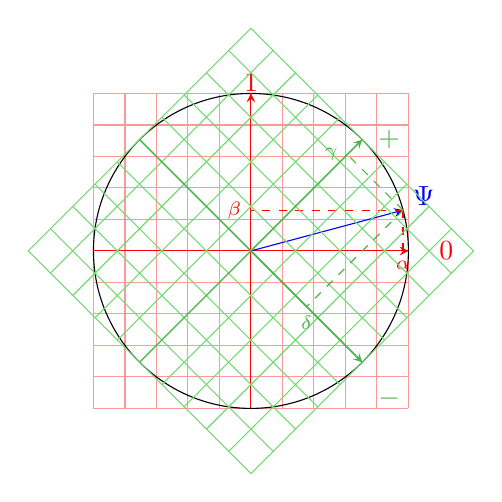
\begin{tikzpicture}
\def\vectsize{.7}
\def\radius{5cm}
\def\labelrad{6.2cm}
\def\ketrad{6.2cm}
\def\arrowrad{3cm}

\def\ojfrangle{0}
\def\ojobangle{15}
\def\ojscale{.4}
\begin{scope}[scale=\ojscale, rotate=\ojfrangle]
\draw[thin,red!40] (-5,-5) grid (5,5);
\draw (0,0) circle (\radius);
\draw [thin, red](-5,0)--(5,0);
\draw [thin, red](0,-5) -- (0,5);
\draw[red, -stealth](0,0)--(0,\radius);
\draw[red, -stealth](0,0)--(\radius,0);
\draw[blue, -stealth](0,0) -- (\ojobangle:\radius) node[right, yshift=5]{$\ket{\Psi}$};
\draw[dashed, red](\radius*cos{\ojobangle},\radius*sin{\ojobangle} ) -- (\radius*cos{\ojobangle}, 0) node[below, xshift=0]{${\scriptstyle \alpha}$};

\draw[dashed, red](\radius*cos{\ojobangle},\radius*sin{\ojobangle} ) -- (0, \radius*sin{\ojobangle}) node[ left, xshift=0]{${\scriptstyle \beta}$};


%\node[scale=1] at (-2,8) {Eenheidscirkel}; 
\node[scale=1, label={[red, yshift=-20]$\ket{1}$}]
      at ( 90:\ketrad) {};
\node[scale=1, label={[red, yshift=-10]$\ket{0}$}]
      at (  0:\ketrad) {};
\end{scope}
\def\ojfrangle{-45}
\def\ojobangle{15}
\def\ojscale{.4}
\begin{scope}[scale=\ojscale, rotate=\ojfrangle]
\draw[thin,green!40!lightgray] (-5,-5) grid (5,5);
%\draw[yellow] (0,0) circle (\radius);
\draw [green!40!gray](-5,0)--(5,0);
\draw [green!40!gray](0,-5) -- (0,5);
\draw[green!40!gray, -stealth](0,0)--(0,\radius);
\draw[green!40!gray, -stealth](0,0)--(\radius,0);
%\node at (0,0) (o) {};
%\node at (0,15:\radius) (p) {$P$};
\draw[dashed, green!40!gray]
     ({\radius*sin{(-\ojobangle-\ojfrangle)}},{\radius*cos{(-\ojobangle-\ojfrangle)}})--
     ({\radius*sin{(-\ojobangle-\ojfrangle)}},0)
     node[below, xshift=0]
     {${\scriptstyle \delta}$};
\draw[dashed, green!40!gray]
     ({\radius*sin{(-\ojobangle-\ojfrangle)}},{\radius*cos{(-\ojobangle-\ojfrangle)}})--
     (0,{\radius*cos{(-\ojobangle-\ojfrangle)}})
     node[ left, xshift=0]
     {${\scriptstyle \gamma}$};

\node[scale=1, label={[green!40!gray, yshift=-20]$\ket{+}$}] 
     at ( 90:\ketrad) {};
\node[scale=1, label={[green!40!gray, yshift=-14]$\ket{-}$}]
     at (  0:\ketrad) {};
\end{scope}
\end{tikzpicture}
%\captionof{figure}{Eenheidscirkel. met eenheidsvecotoren $\ket{0}$ en $\ket{1}$. \label{fig:unitc}}

\end{minipage}%
\hfill
\begin{minipage}{.45\textwidth}
\captionof{figure}{De vector $\Psi$ (blauw) wordt in de  standaardbasis (rood) genoteerd als $\Psi_s=\alpha\ket{0}+\beta\ket{1}$ en in de  diagonale basis (groen)  als $\Psi_d=\gamma\ket{+}+\delta\ket{-}$.}\label{fig:twobases}
\end{minipage}
%\caption{E\'en vector in standaardbasis (rood) en diagonale basis.}\label{fig:hvad}
%\end{figure}
\end{flushleft}


Dit figuur maakt nog eens duidelijk dat de beschrijving van een toestand van een qubit door middel van amplitudes altijd afhangt van de instelling van het meetapparaat.

\end{document}